\begin{figure}[!ht]
    \captionsetup{labelformat=empty}
    \centering
    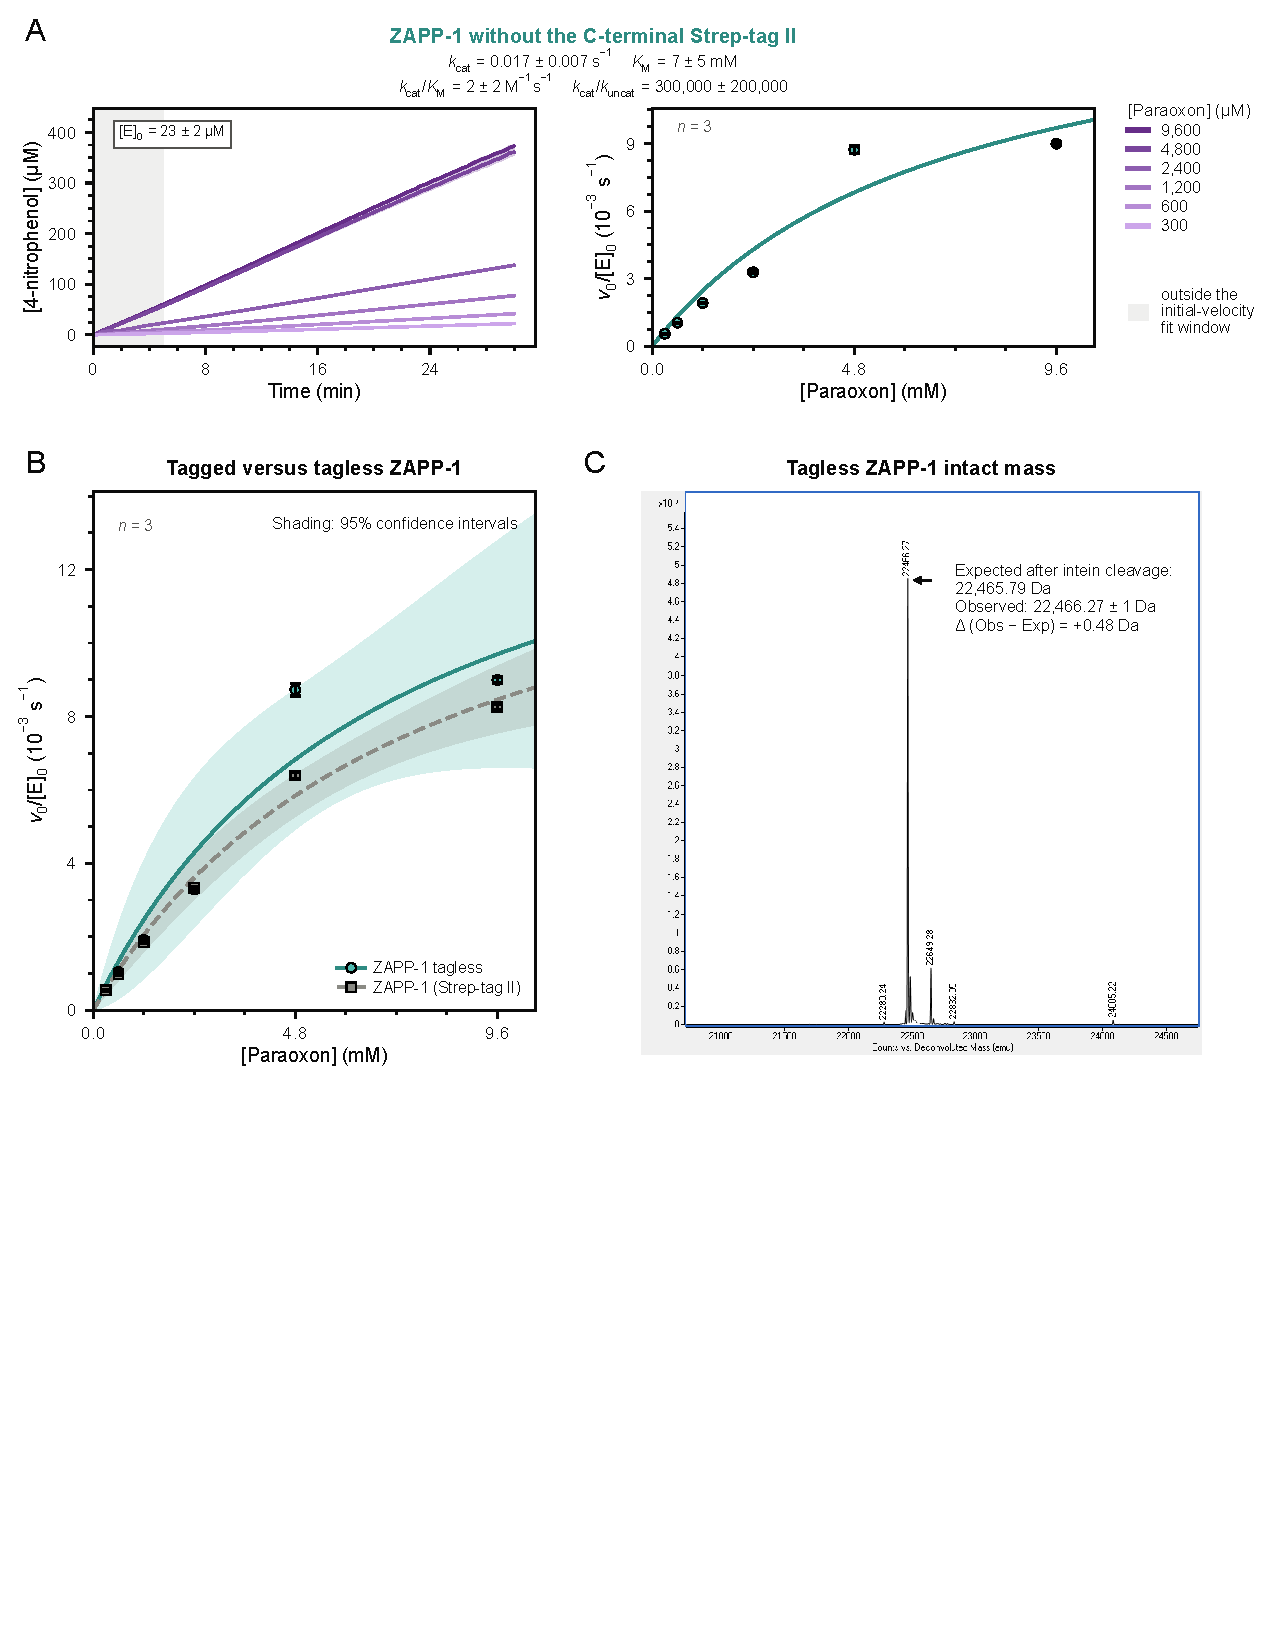
\includegraphics[width=1.0\linewidth]{PTE__v2SI__ZAPP1_tagless.pdf}
    \caption{}
\end{figure}
\clearpage

\begin{figure}[!ht]
    \captionsetup{labelformat=adja-page}
    \ContinuedFloat
    \centering
    \caption{
        \textbf{ZAPP-1 activity does not require the C-terminal Strep-tag II.}
        \textbf{A}, Background-corrected progress curves (left) and Michaelis--Menten fit (right) for tagless ZAPP-1 ($[E]_0 = 23.4$~$\mu$M; 0.3--9.6~mM paraoxon, 25~mM NaHCO$_3$, 25~$\degree$C). Curves are colored by substrate concentration; the shaded regions around progress curves and the error bars on mean velocities show the s.e.m. of three technical replicates. The gray band marks the interval excluded from initial-velocity fitting; velocities were fit from 300 to 1800~s. Parameter uncertainties were calculated as described in Methods, and $k_{\mathrm{cat}}/k_{\mathrm{uncat}}$ uses the bicarbonate-supplemented uncatalyzed rate (\cref{fig:PTE_v2SI_kuncat}).
        \textbf{B}, Overlay of the tagless fit (teal) and the Strep-tag II-containing ZAPP-1 reference fit (gray; $[E]_0 = 24.0$~$\mu$M; \cref{fig:PTE_v2SI_kinetics_round1}). Shading denotes approximate pointwise 95\% confidence intervals for the fitted mean response, calculated as described in Methods. Tagless ZAPP-1 retained comparable catalytic activity to the Strep-tagged protein ($k_{\mathrm{cat}} \approx 0.017$ versus $0.015$~s$^{-1}$), with overlapping 95\% confidence intervals for the fitted Michaelis--Menten curves. These results demonstrate that activity does not require the C-terminal Strep-tag II and suggest that tag removal has little effect under the conditions tested.
        \textbf{C}, Deconvoluted intact-protein ESI-MS spectrum of tagless ZAPP-1. The principal peak at 22466.27~Da agrees with the expected average mass of 22465.79~Da for the 203-residue protein after intein cleavage. The observed--expected difference ($\Delta m = +0.48$~Da) is within the approximate measurement uncertainty of $\pm 1$~Da.
    }
    \label{fig:PTE_v2SI_ZAPP1_tagless}
\end{figure}
\clearpage
